% ============================================================================
% TOPIC 18D: MOLECULAR COLLISION DYNAMICS
% ============================================================================

\section{Topic 18D: Molecular Collision Dynamics}

% ===========================================================================
% Slide: Topic 18D Overview
% ===========================================================================
\begin{frame}{Topic 18D: Overview}

\textbf{Zooming in to the Molecular Level}

\vspace{0.3cm}

\begin{itemize}
    \item \textbf{Goal:} Understand exactly what happens during a single collision.
    \item \textbf{Experiment:} Molecular Beams.
    \item \textbf{Theory:} Potential Energy Surfaces (PES) and Trajectories.
\end{itemize}

\vspace{0.3cm}
\textbf{Key Questions:}
\begin{itemize}
    \item How does energy distribution affect reactivity?
    \item In what direction do products fly away?
    \item What is the detailed reaction path?
    \item How does energy partition between products?
\end{itemize}

\vspace{0.3cm}
\textbf{Pioneers:} Herschbach, Lee, Polanyi (Nobel Prize 1986)

\end{frame}

% ===========================================================================
% Slide: Why Molecular Beams?
% ===========================================================================
\begin{frame}{Why Molecular Beams?}

\textbf{Problem with Bulk Gas Experiments:}

\begin{itemize}
    \item Multiple collisions
    \item Maxwell-Boltzmann distribution of velocities
    \item Difficult to isolate single reactive event
    \item Cannot control initial conditions precisely
\end{itemize}

\vspace{0.3cm}
\textbf{Molecular Beam Advantages:}

\begin{itemize}
    \item \alert{Single collision} conditions (high vacuum, $\sim 10^{-6}$ torr)
    \item \alert{Control} of velocity, quantum states, collision angle
    \item \alert{Measure} angular distribution of products
    \item \alert{Detect} product quantum states (vibrational, rotational)
    \item \alert{State-to-state} chemistry: A(v,J) + B → C(v',J') + D
\end{itemize}

\end{frame}

% ===========================================================================
% Slide: Molecular Beams - Basic Setup
% ===========================================================================
\begin{frame}{Molecular Beams - Experimental Setup}

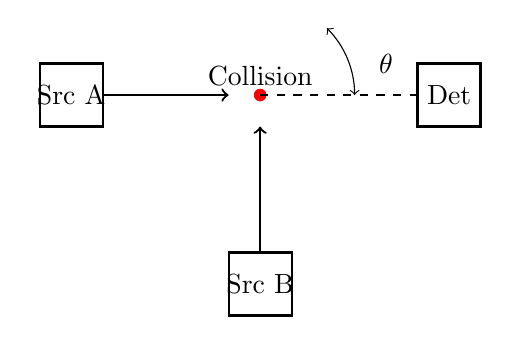
\begin{tikzpicture}[scale=0.8]
    % Source A
    \draw[thick] (-5,1) rectangle (-4,2);
    \node at (-4.5,1.5) {Src A};
    \draw[->, thick] (-4,1.5) -- (-2,1.5);

    % Source B
    \draw[thick] (-2,-2) rectangle (-1,-1);
    \node at (-1.5,-1.5) {Src B};
    \draw[->, thick] (-1.5,-1) -- (-1.5,1);

    % Collision Zone
    \fill[red] (-1.5,1.5) circle (0.1cm);
    \node at (-1.5,1.8) {Collision};

    % Detector
    \draw[thick] (1,1) rectangle (2,2);
    \node at (1.5,1.5) {Det};
    \draw[dashed] (-1.5,1.5) -- (1,1.5);
    \draw[<->] (0,1.5) arc (0:45:1.5);
    \node at (0.5,2) {$\theta$};
\end{tikzpicture}

\vspace{0.3cm}
\textbf{Components:}
\begin{itemize}
    \item \textbf{Sources:} Supersonic expansion (velocity selection)
    \item \textbf{Collision Zone:} Crossed beams at controlled angle
    \item \textbf{Detector:} Mass spectrometer + time-of-flight (TOF) analysis
    \item \textbf{Vacuum:} $10^{-6}$ to $10^{-8}$ torr to prevent multiple collisions
\end{itemize}

\end{frame}

% ===========================================================================
% Slide: Velocity Selection
% ===========================================================================
\begin{frame}{Velocity Selection: Supersonic Expansion}

\textbf{Technique:} Gas expands through small nozzle into vacuum

\begin{columns}[T]
\column{0.5\textwidth}
\textbf{Before Expansion:}
\begin{itemize}
    \item Maxwell-Boltzmann distribution
    \item $T \sim 300$ K
    \item Wide velocity spread
\end{itemize}

\vspace{0.3cm}
\textbf{After Expansion:}
\begin{itemize}
    \item Narrow velocity distribution
    \item Effective $T \sim 1$-$10$ K
    \item All molecules move with $v \approx \bar{v}$
\end{itemize}

\column{0.5\textwidth}
\centering
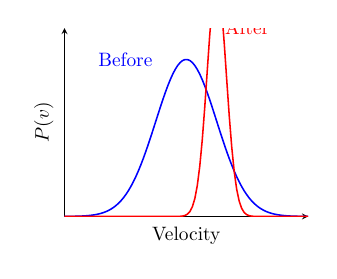
\begin{tikzpicture}[scale=0.7]
    \begin{axis}[
        xlabel={Velocity},
        ylabel={$P(v)$},
        xtick=\empty,
        ytick=\empty,
        axis lines=left,
        width=6cm,
        height=5cm,
        ymin=0, ymax=1.2
    ]
    % Broad distribution
    \addplot[blue, thick, domain=0:4, samples=100] {exp(-(x-2)^2/0.5)};
    \node[blue] at (axis cs:1,1) {Before};

    % Narrow distribution
    \addplot[red, thick, domain=0:4, samples=100] {1.5*exp(-(x-2.5)^2/0.05)};
    \node[red] at (axis cs:3,1.2) {After};
    \end{axis}
\end{tikzpicture}
\end{columns}

\textbf{Result:} Collision energy is well-defined!

\end{frame}

% ===========================================================================
% Slide: Collision Energy
% ===========================================================================
\begin{frame}{Collision Energy and Impact Parameter}

\textbf{Center-of-Mass Energy:}

For two molecules with velocities $\vec{v}_A$ and $\vec{v}_B$:

\keyeq{E_{\text{coll}} = \frac{1}{2}\mu v_{\text{rel}}^2}

where $\mu = \frac{m_A m_B}{m_A + m_B}$ is reduced mass.

\vspace{0.3cm}
\textbf{Impact Parameter $b$:}

\begin{columns}[T]
\column{0.6\textwidth}
\begin{itemize}
    \item Distance of closest approach if no interaction
    \item Small $b$: Head-on collision
    \item Large $b$: Grazing collision
    \item Maximum $b$ for reaction: $b_{\text{max}}$
    \item Reactive cross-section: $\sigma_r = \pi b_{\text{max}}^2$
\end{itemize}

\column{0.4\textwidth}
\centering
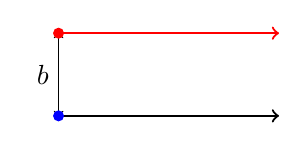
\begin{tikzpicture}[scale=0.7]
    \draw[->, thick] (0,0) -- (4,0);
    \draw[->, thick, red] (0,1.5) -- (4,1.5);
    \draw[<->] (0,0) -- (0,1.5) node[midway, left] {$b$};
    \fill[blue] (0,0) circle (0.1cm);
    \fill[red] (0,1.5) circle (0.1cm);
\end{tikzpicture}
\end{columns}

\end{frame}

% ===========================================================================
% Slide: Differential Cross-Section
% ===========================================================================
\begin{frame}{Differential Cross-Section}

\begin{columns}[T]
\column{0.55\textwidth}
\textbf{Definition:}

We measure the \textbf{Differential Cross-Section} $\sigma(\theta, \phi)$:

\keyeq{dN = \sigma(\theta, \phi) I_{\text{inc}} d\Omega}

\begin{itemize}
    \item $dN$: Particles scattered into $d\Omega$
    \item $I_{\text{inc}}$: Incident flux
    \item $\sigma(\theta)$: Angular cross-section
    \item Units: area/steradian (Å$^2$/sr)
\end{itemize}

\vspace{0.2cm}
\textbf{Information Content:}
\begin{itemize}
    \item Scattering probability vs angle
    \item Forces during collision
    \item Reaction mechanism
\end{itemize}

\column{0.45\textwidth}
\centering
\includegraphics[width=\textwidth]{Reaction_Dynamics_Interactive/images/differential_cross_section_polar.png}

\vspace{0.1cm}
\tiny \textit{Explore molecular beams interactively}

\end{columns}

\end{frame}

% ===========================================================================
% Slide: Scattering Patterns
% ===========================================================================
\begin{frame}{Types of Scattering Patterns}

\begin{columns}[T]
\column{0.5\textwidth}
\textbf{Forward Scattering ($\theta \approx 0°$):}
\begin{itemize}
    \item "Stripping" mechanism
    \item Grazing collision (large $b$)
    \item Fast, direct reaction
    \item Example: K + Br$_2$ → KBr + Br
    \item Products fly forward
\end{itemize}

\column{0.5\textwidth}
\textbf{Backward Scattering ($\theta \approx 180°$):}
\begin{itemize}
    \item "Rebound" mechanism
    \item Head-on collision (small $b$)
    \item Strong repulsive interaction
    \item Example: K + CH$_3$I
    \item Products bounce back
\end{itemize}
\end{columns}

\vspace{0.3cm}
\textbf{Sideways Scattering ($\theta \approx 90°$):}
\begin{itemize}
    \item Complex formation
    \item Long-lived intermediate
    \item Symmetric angular distribution
\end{itemize}

\end{frame}

% ===========================================================================
% Slide: Newton Diagram
% ===========================================================================
\begin{frame}{Newton Diagram}

\textbf{Relating Lab Frame to Center-of-Mass Frame:}

\begin{center}
\begin{tikzpicture}[scale=0.8]
    % CM circle
    \draw[thick, blue] (0,0) circle (2cm);
    \node[blue] at (0,-2.5) {CM Frame};

    % Lab velocity
    \draw[->, thick, red] (0,0) -- (3,0) node[right] {$\vec{v}_{\text{CM}}$};
    \node[red] at (3.5,-0.5) {Lab Frame};

    % Product velocity in CM
    \draw[->, thick] (0,0) -- (1.4,1.4) node[above left] {$\vec{v}_{\text{CM}}^{\text{prod}}$};

    % Product velocity in Lab
    \draw[->, thick, darkgreen] (0,0) -- (4.4,1.4) node[above] {$\vec{v}_{\text{Lab}}^{\text{prod}}$};

    \draw[dashed] (1.4,1.4) -- (4.4,1.4);
    \draw[<->] (0.5,0) arc (0:45:0.5);
    \node at (0.7,0.3) {$\theta_{\text{CM}}$};
\end{tikzpicture}
\end{center}

\[ \vec{v}_{\text{Lab}} = \vec{v}_{\text{CM}}^{\text{prod}} + \vec{v}_{\text{CM}} \]

Detector measures lab angles; theory predicts CM angles.

\end{frame}

% ===========================================================================
% Slide: State-to-State Chemistry - Part 1
% ===========================================================================
\begin{frame}{State-to-State Chemistry (Part 1)}

\textbf{Modern Achievement:} Prepare reactants in specific quantum states and measure product states.

\vspace{0.5cm}
\textbf{Example:} H + D$_2$(v=0, J=0) → HD(v', J') + D

\begin{itemize}
    \item Prepare D$_2$ in ground vibrational and rotational state
    \item Measure HD product distribution over v' and J'
    \item Map out complete energy disposal
\end{itemize}

\vspace{0.5cm}
\textbf{Advantages:}
\begin{itemize}
    \item Most detailed information possible
    \item Direct test of theory
    \item Reveals quantum effects
\end{itemize}

\end{frame}

% ===========================================================================
% Slide: State-to-State Chemistry - Part 2
% ===========================================================================
\begin{frame}{State-to-State Chemistry (Part 2)}

\textbf{Experimental Techniques:}
\begin{itemize}
    \item \textbf{State preparation:} Laser excitation, Stark/Zeeman selection
    \item \textbf{State detection:} Laser-induced fluorescence (LIF), REMPI
\end{itemize}

\vspace{0.5cm}
\textbf{Ultimate Goal:} Complete characterization:
\[ \sigma(E_{\text{coll}}, v, J, b \to v', J', \theta, \phi) \]

This is the \alert{full quantum scattering matrix}!

\vspace{0.5cm}
\textbf{Challenge:} Enormous amount of data, but worth it for fundamental understanding

\end{frame}

% ===========================================================================
% Slide: Potential Energy Surfaces (PES)
% ===========================================================================
\begin{frame}{Potential Energy Surfaces (PES)}

\textbf{The Landscape of Reaction}

\begin{itemize}
    \item Plot Potential Energy $V$ vs. atomic coordinates.
    \item For A + BC $\to$ AB + C (collinear):
        \item Axes: $R_{AB}$ and $R_{BC}$.
\end{itemize}

\vspace{0.2cm}
\centering
\includegraphics[width=0.7\textwidth]{Reaction_Dynamics_Interactive/images/pes_contour_leps.png}

\vspace{0.1cm}
{\small LEPS Potential Energy Surface for A + BC $\to$ AB + C}

\vspace{0.1cm}
\textbf{Reality:} 3N-6 dimensions for N atoms (reduced to 2D for collinear triatomics)

\end{frame}

% ===========================================================================
% Slide: Calculating PES - Part 1
% ===========================================================================
\begin{frame}{How to Calculate PES (Part 1)}

\textbf{Theoretical Methods:}

\begin{enumerate}
    \item \textbf{Ab Initio Quantum Chemistry:}
        \begin{itemize}
            \item Solve Schrödinger equation for electrons
            \item Born-Oppenheimer approximation (nuclei fixed)
            \item Methods: HF, MP2, CCSD(T), CASSCF
            \item Very accurate but computationally expensive
        \end{itemize}

    \item \textbf{Density Functional Theory (DFT):}
        \begin{itemize}
            \item Faster than ab initio
            \item Good accuracy for many systems
            \item Functionals: B3LYP, M06-2X, $\omega$B97X-D
        \end{itemize}
\end{enumerate}

\end{frame}

% ===========================================================================
% Slide: Calculating PES - Part 2
% ===========================================================================
\begin{frame}{How to Calculate PES (Part 2)}

\textbf{Theoretical Methods (continued):}

\begin{enumerate}
    \setcounter{enumi}{2}
    \item \textbf{Semi-Empirical/Fitted:}
        \begin{itemize}
            \item LEPS (London-Eyring-Polanyi-Sato)
            \item Fit to experimental data
            \item Fast but less accurate
        \end{itemize}
\end{enumerate}

\vspace{0.5cm}
\textbf{Trade-offs:}
\begin{itemize}
    \item Accuracy vs. computational cost
    \item Ab initio: Most accurate, most expensive
    \item DFT: Good balance for most systems
    \item Semi-empirical: Fast screening, less reliable
\end{itemize}

\end{frame}

% ===========================================================================
% Slide: Features of PES
% ===========================================================================
\begin{frame}{Features of PES}

\begin{columns}[T]
\column{0.5\textwidth}
\begin{itemize}
    \item \textbf{Reactant Valley:} A far from BC.
    \item \textbf{Product Valley:} AB far from C.
    \item \textbf{Saddle Point:} The Transition State.
        \item Maximum along reaction path.
        \item Minimum perpendicular to path.
    \item \textbf{Reaction Path:} Minimum energy route (MEP).
    \item \textbf{Barrier Height:} Energy at saddle point.
\end{itemize}

\column{0.5\textwidth}
\centering
% Simplified diagram
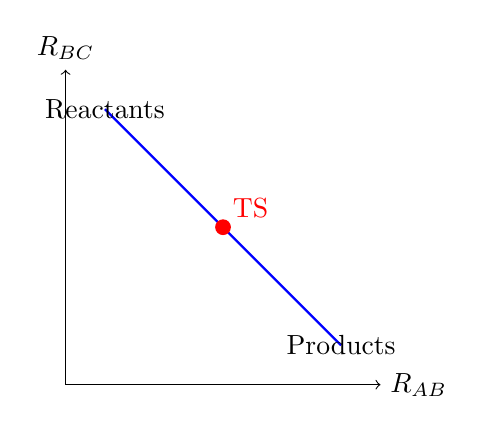
\begin{tikzpicture}
    \draw[->] (0,0) -- (4,0) node[right] {$R_{AB}$};
    \draw[->] (0,0) -- (0,4) node[above] {$R_{BC}$};
    \draw[thick, blue] (0.5,3.5) to[out=-45,in=135] (3.5,0.5);
    \node at (0.5,3.5) {Reactants};
    \node at (3.5,0.5) {Products};
    \fill[red] (2,2) circle (0.1cm) node[above right] {TS};
\end{tikzpicture}
\end{columns}

\vspace{0.3cm}
\textbf{Intrinsic Reaction Coordinate (IRC):} Path of steepest descent from TS to reactants and products.

\end{frame}

% ===========================================================================
% Slide: Classical Trajectories - Part 1
% ===========================================================================
\begin{frame}{Classical Trajectory Calculations (Part 1)}

\textbf{Method:} Solve Newton's equations on the PES

\begin{enumerate}
    \item Start with initial conditions: positions, velocities, $E_{\text{coll}}$, $b$
    \item Calculate forces: $\vec{F}_i = -\nabla_i V(\vec{R})$
    \item Integrate equations of motion: $m_i \ddot{\vec{R}}_i = \vec{F}_i$
    \item Follow trajectory until products separate
    \item Record: reaction outcome, scattering angle, product energies
\end{enumerate}

\end{frame}

% ===========================================================================
% Slide: Classical Trajectories - Part 2
% ===========================================================================
\begin{frame}{Classical Trajectory Calculations (Part 2)}

\textbf{Statistical Analysis:}
\begin{itemize}
    \item Run thousands of trajectories
    \item Sample different $b$ and initial conditions
    \item Calculate average cross-sections, energy distributions
\end{itemize}

\vspace{0.5cm}
\textbf{Limitations:}
\begin{itemize}
    \item Classical mechanics (no tunneling)
    \item Can violate zero-point energy (ZPE)
    \item No quantum interference effects
    \item Need ZPE constraints for realistic simulations
\end{itemize}

\vspace{0.5cm}
\textbf{When to use:} Heavy atoms, high energies, statistical averaging

\end{frame}

% ===========================================================================
% Slide: Trajectory Example
% ===========================================================================
\begin{frame}{Trajectory Example: H + H$_2$ → H$_2$ + H}

\begin{center}
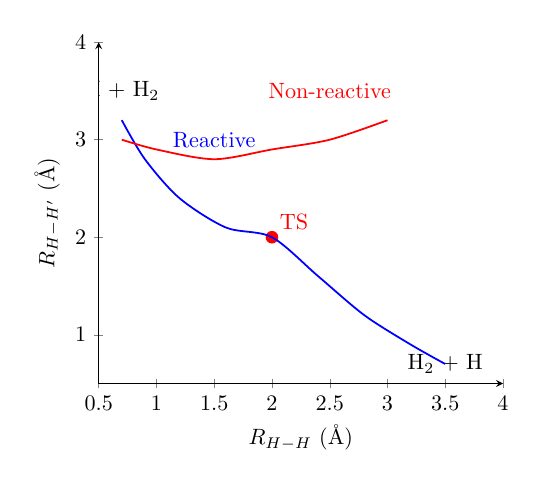
\begin{tikzpicture}[scale=0.8]
    \begin{axis}[
        xlabel={$R_{\text{H-H}}$ (Å)},
        ylabel={$R_{\text{H-H'}}$ (Å)},
        xmin=0.5, xmax=4,
        ymin=0.5, ymax=4,
        axis lines=left,
        width=8cm,
        height=7cm
    ]
    % Reactant valley
    \node at (axis cs:0.7,3.5) {H + H$_2$};
    % Product valley
    \node at (axis cs:3.5,0.7) {H$_2$ + H};
    % TS region
    \fill[red] (axis cs:2,2) circle (0.1cm) node[above right] {TS};

    % Reactive trajectory
    \addplot[blue, thick, smooth] coordinates {
        (0.7,3.2) (0.9,2.8) (1.2,2.4) (1.6,2.1) (2.0,2.0) (2.4,1.6) (2.8,1.2) (3.2,0.9) (3.5,0.7)
    };
    \node[blue] at (axis cs:1.5,3) {Reactive};

    % Non-reactive trajectory
    \addplot[red, thick, smooth] coordinates {
        (0.7,3.0) (1.0,2.9) (1.5,2.8) (2.0,2.9) (2.5,3.0) (3.0,3.2)
    };
    \node[red] at (axis cs:2.5,3.5) {Non-reactive};
    \end{axis}
\end{tikzpicture}
\end{center}

Blue: Passes through TS region → reaction. Red: Turns back → no reaction.

\end{frame}

% ===========================================================================
% Slide: Product Energy Distribution
% ===========================================================================
\begin{frame}{Product Energy Distribution}

\textbf{Where does the energy go?}

Total available energy: $E_{\text{avail}} = E_{\text{coll}} + \Delta H_{\text{rxn}}$

\textbf{Partitioning:}
\begin{itemize}
    \item \textbf{Translation:} $E_{\text{trans}}$ (kinetic energy of products flying apart)
    \item \textbf{Vibration:} $E_{\text{vib}}$ (internal vibration of product molecules)
    \item \textbf{Rotation:} $E_{\text{rot}}$ (molecular rotation)
\end{itemize}

\keyeq{E_{\text{avail}} = E_{\text{trans}} + E_{\text{vib}} + E_{\text{rot}}}

\vspace{0.3cm}
\textbf{Distribution depends on PES topology:}
\begin{itemize}
    \item Attractive surface → vibrationally "hot" products
    \item Repulsive surface → translationally "hot" products
\end{itemize}

\end{frame}

% ===========================================================================
% Slide: Attractive vs. Repulsive Surfaces
% ===========================================================================
\begin{frame}{Attractive vs. Repulsive Surfaces}

\textbf{Where is the barrier located?}

\begin{columns}[T]
\column{0.5\textwidth}
\textbf{Attractive (Early Barrier):}
\begin{itemize}
    \item Barrier in reactant valley
    \item TS resembles reactants
    \item \alert{Translational energy} helps cross barrier
    \item Products are \alert{vibrationally excited}
    \item Example: K + Br$_2$ (Harpoon reaction)
    \item Energy flows: Translation → Vibration
\end{itemize}

\column{0.5\textwidth}
\textbf{Repulsive (Late Barrier):}
\begin{itemize}
    \item Barrier in product valley
    \item TS resembles products
    \item \alert{Vibrational energy} helps cross barrier
    \item Products are \alert{translationally excited}
    \item Example: H + Cl$_2$
    \item Energy flows: Vibration → Translation
\end{itemize}
\end{columns}

\end{frame}

% ===========================================================================
% Slide: Polanyi's Rules - Part 1
% ===========================================================================
\begin{frame}{Polanyi's Rules (Part 1)}

\emphbox{
\textbf{Polanyi's Rule 1:} For reactions with early barriers, translational energy is more effective than vibrational energy in promoting reaction.
}

\emphbox{
\textbf{Polanyi's Rule 2:} For reactions with late barriers, vibrational energy is more effective than translational energy in promoting reaction.
}

\vspace{0.5cm}
\textbf{Key Insight:} The location of the barrier determines which type of energy is most effective.

\end{frame}

% ===========================================================================
% Slide: Polanyi's Rules - Part 2
% ===========================================================================
\begin{frame}{Polanyi's Rules (Part 2)}

\textbf{Intuitive Explanation:}
\begin{itemize}
    \item \textbf{Early Barrier:} Need speed to "run up" the entrance valley before bonds rearrange.
    \item \textbf{Late Barrier:} Need stretched bonds (vibration) to help make the turn into the product valley.
\end{itemize}

\vspace{0.5cm}
\textbf{Experimental Verification:}
\begin{itemize}
    \item Compare $\sigma_r(E_{\text{trans}}, v=0)$ vs. $\sigma_r(E_{\text{trans}}, v=1)$
    \item Prepare reactants with vibrational excitation
    \item Measure which form of energy enhances reactivity more
\end{itemize}

\vspace{0.5cm}
\textbf{Impact:} Guide for controlling chemical reactions with laser excitation

\end{frame}

% ===========================================================================
% Slide: Energy Disposal
% ===========================================================================
\begin{frame}{Energy Disposal: Surprisal Analysis}

\textbf{Question:} How does actual product energy distribution compare to statistical expectation?

\textbf{Statistical (Phase Space) Prediction:}
\begin{itemize}
    \item Assume all product states equally accessible
    \item Predict: $P_{\text{stat}}(v') \propto \rho(E_{\text{avail}} - E_{v'})$
    \item Density of states $\rho$ increases with energy
\end{itemize}

\vspace{0.3cm}
\textbf{Surprisal:}
\keyeq{I(v') = -\ln\left(\frac{P_{\text{obs}}(v')}{P_{\text{stat}}(v')}\right)}

\begin{itemize}
    \item $I(v') > 0$: Less than statistical (vibration "starved")
    \item $I(v') < 0$: More than statistical (vibration "enhanced")
\end{itemize}

\textbf{Reveals:} Direct vs. complex mechanism

\end{frame}

% ===========================================================================
% Slide: Harpoon Mechanism - Part 1
% ===========================================================================
\begin{frame}{Harpoon Mechanism: K + Br$_2$ → KBr + Br (Part 1)}

\textbf{Classic Example of Attractive Surface}

\vspace{0.3cm}
\textbf{Mechanism:}
\begin{enumerate}
    \item At large distance ($R \sim 6$ Å): Electron jumps from K to Br$_2$
        \[ \text{K} + \text{Br}_2 \to \text{K}^+ + \text{Br}_2^- \]
    \item Coulomb attraction pulls ions together (fast!)
    \item K$^+$ approaches Br$_2^-$, forming KBr$^-$ complex
    \item Br$^-$ leaves with high kinetic energy
\end{enumerate}

\end{frame}

% ===========================================================================
% Slide: Harpoon Mechanism - Part 2
% ===========================================================================
\begin{frame}{Harpoon Mechanism: K + Br$_2$ → KBr + Br (Part 2)}

\textbf{Experimental Observations:}
\begin{itemize}
    \item Very large cross-section: $\sigma \sim 200$ Å$^2$ (vs. $\sim 10$ Å$^2$ typical)
    \item Forward scattering (stripping mechanism)
    \item KBr product highly vibrationally excited
    \item Low activation energy
\end{itemize}

\vspace{0.5cm}
\textbf{Why "Harpoon"?}
\begin{itemize}
    \item Electron "thrown" from K at long range
    \item Like harpooning a whale from distance
    \item Ionic attraction then "reels in" the reactants
    \item Fast, efficient reaction
\end{itemize}

\end{frame}

% ===========================================================================
% Slide: Spectator Stripping
% ===========================================================================
\begin{frame}{Spectator Stripping}

\textbf{Mechanism:} In A + BC → AB + C, atom C is a "spectator"

\begin{columns}[T]
\column{0.6\textwidth}
\textbf{Characteristics:}
\begin{itemize}
    \item Fast, direct reaction
    \item C atom barely affected
    \item AB bond forms while BC bond breaks
    \item High impact parameter (grazing collision)
    \item Forward scattering
    \item C "stripped off" from BC
\end{itemize}

\vspace{0.3cm}
\textbf{Example:} K + CH$_3$I → KI + CH$_3$
\begin{itemize}
    \item CH$_3$ group acts as spectator
    \item KI formed in collision zone
    \item CH$_3$ continues forward with little deflection
\end{itemize}

\column{0.4\textwidth}
\centering
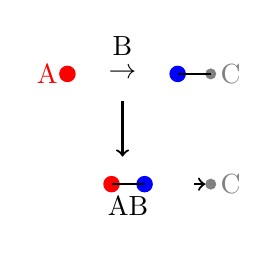
\begin{tikzpicture}[scale=0.7]
    % Before
    \fill[red] (0,2) circle (0.15cm) node[left] {A};
    \fill[blue] (2,2) circle (0.15cm);
    \fill[gray] (2.6,2) circle (0.1cm) node[right] {C};
    \draw[thick] (2,2) -- (2.6,2);
    \node at (1,2) {$\to$};
    \node at (1,2.5) {B};

    % Arrow
    \draw[->, thick] (1,1.5) -- (1,0.5);

    % After
    \fill[red] (0.8,0) circle (0.15cm);
    \fill[blue] (1.4,0) circle (0.15cm);
    \draw[thick] (0.8,0) -- (1.4,0);
    \node at (1.1,-0.4) {AB};

    \fill[gray] (2.6,0) circle (0.1cm) node[right] {C};
    \draw[->, thick] (2.3,0) -- (2.5,0);
\end{tikzpicture}
\end{columns}

\end{frame}

% ===========================================================================
% Slide: Quantum Effects - Part 1
% ===========================================================================
\begin{frame}{Quantum Effects in Dynamics (Part 1)}

\textbf{When Classical Trajectories Fail:}

\begin{enumerate}
    \item \textbf{Tunneling:}
        \begin{itemize}
            \item Light atoms (H, D) can tunnel through barriers
            \item Important for H-transfer reactions
            \item Classical: $k = 0$ below barrier; Quantum: $k > 0$
        \end{itemize}

    \item \textbf{Zero-Point Energy (ZPE):}
        \begin{itemize}
            \item Molecules have ZPE = $\frac{1}{2}h\nu$ even at $v=0$
            \item Classical trajectories can violate ZPE
            \item Need ZPE constraints in classical simulations
        \end{itemize}
\end{enumerate}

\end{frame}

% ===========================================================================
% Slide: Quantum Effects - Part 2
% ===========================================================================
\begin{frame}{Quantum Effects in Dynamics (Part 2)}

\textbf{When Classical Trajectories Fail (continued):}

\begin{enumerate}
    \setcounter{enumi}{2}
    \item \textbf{Resonances:}
        \begin{itemize}
            \item Quasi-bound states in complex region
            \item Show up as oscillations in $\sigma_r(E)$
            \item Pure quantum effect (interference)
        \end{itemize}

    \item \textbf{Quantized Product States:}
        \begin{itemize}
            \item Classical: continuous energy distribution
            \item Quantum: discrete vibrational/rotational levels
        \end{itemize}
\end{enumerate}

\vspace{0.5cm}
\textbf{Bottom Line:} Quantum dynamics needed for light atoms, low energies, or detailed state-to-state studies.

\end{frame}

% ===========================================================================
% Slide: Worked Example 1
% ===========================================================================
\begin{frame}{Worked Example 1: Collision Energy}

\textbf{Problem:} In a crossed molecular beam experiment, H atoms (mass = 1 amu) with velocity 2000 m/s collide with D$_2$ molecules (mass = 4 amu) at rest. Calculate the collision energy.

\vspace{0.3cm}
\textbf{Solution:}

Step 1: Calculate reduced mass
\[ \mu = \frac{m_{\text{H}} \cdot m_{\text{D}_2}}{m_{\text{H}} + m_{\text{D}_2}} = \frac{1 \times 4}{1 + 4} = 0.8 \text{ amu} \]

Convert to kg: $\mu = 0.8 \times 1.66 \times 10^{-27} = 1.33 \times 10^{-27}$ kg

Step 2: Relative velocity
\[ v_{\text{rel}} = v_{\text{H}} - v_{\text{D}_2} = 2000 - 0 = 2000 \text{ m/s} \]

Step 3: Collision energy
\[ E_{\text{coll}} = \frac{1}{2}\mu v_{\text{rel}}^2 = \frac{1}{2}(1.33 \times 10^{-27})(2000)^2 = 2.66 \times 10^{-21} \text{ J} \]

\keyeq{E_{\text{coll}} = 0.016 \text{ eV} = 1.55 \text{ kJ/mol}}

\end{frame}

% ===========================================================================
% Slide: Worked Example 2
% ===========================================================================
\begin{frame}{Worked Example 2: Reactive Cross-Section}

\textbf{Problem:} For the reaction H + D$_2$ → HD + D, the maximum impact parameter for reaction at $E_{\text{coll}} = 0.5$ eV is $b_{\text{max}} = 1.8$ Å. Calculate:
\begin{enumerate}[a)]
    \item The reactive cross-section $\sigma_r$
    \item The reaction probability if geometric cross-section is $\sigma_{\text{geom}} = 10$ Å$^2$
\end{enumerate}

\vspace{0.3cm}
\textbf{Solution:}

(a) Reactive cross-section:
\[ \sigma_r = \pi b_{\text{max}}^2 = \pi (1.8)^2 = 10.2 \text{ Å}^2 \]

(b) Reaction probability (opacity function):
\[ P = \frac{\sigma_r}{\sigma_{\text{geom}}} = \frac{10.2}{10} = 1.02 \approx 1.0 \]

\textbf{Interpretation:} At this energy, essentially all collisions within the geometric cross-section lead to reaction (high reactivity).

\end{frame}

% ===========================================================================
% Slide: Worked Example 3
% ===========================================================================
\begin{frame}{Worked Example 3: Energy Partitioning}

\textbf{Problem:} For the reaction F + H$_2$ → HF + H at $E_{\text{coll}} = 0.1$ eV:
\begin{itemize}
    \item $\Delta H_{\text{rxn}} = -1.4$ eV (exothermic)
    \item Measured: HF products have $\langle E_{\text{vib}} \rangle = 1.0$ eV
\end{itemize}

Calculate the average translational and rotational energy of products.

\vspace{0.3cm}
\textbf{Solution:}

Total available energy:
\[ E_{\text{avail}} = E_{\text{coll}} + |\Delta H_{\text{rxn}}| = 0.1 + 1.4 = 1.5 \text{ eV} \]

Energy remaining for translation + rotation:
\[ E_{\text{trans}} + E_{\text{rot}} = E_{\text{avail}} - E_{\text{vib}} = 1.5 - 1.0 = 0.5 \text{ eV} \]

Typical ratio: $E_{\text{rot}} : E_{\text{trans}} \approx 1:2$ (rule of thumb)

\keyeq{E_{\text{rot}} \approx 0.17 \text{ eV}, \quad E_{\text{trans}} \approx 0.33 \text{ eV}}

\textbf{Note:} HF is highly vibrationally excited (67\% into vibration) - characteristic of attractive surface.

\end{frame}

% ===========================================================================
% Slide: Practice Problem 1
% ===========================================================================
\begin{frame}{Practice Problem 1}

\textbf{Problem:} In a crossed beam experiment, Ar atoms (40 amu) with $v = 1500$ m/s collide with O$_2$ molecules (32 amu) with $v = 800$ m/s at 90°. Calculate:

\begin{enumerate}[a)]
    \item The magnitude of the relative velocity
    \item The collision energy in eV
    \item The center-of-mass velocity
\end{enumerate}

\vspace{0.5cm}
\textbf{Answers:}
\begin{itemize}
    \item[(a)] $v_{\text{rel}} = \sqrt{1500^2 + 800^2} = 1700$ m/s
    \item[(b)] $E_{\text{coll}} = 0.17$ eV
    \item[(c)] $v_{\text{CM}} = 1056$ m/s (along Ar beam direction)
\end{itemize}

\end{frame}

% ===========================================================================
% Slide: Practice Problem 2
% ===========================================================================
\begin{frame}{Practice Problem 2}

\textbf{Problem:} For the reaction Cl + HBr → HCl + Br:
\begin{itemize}
    \item Barrier is "late" (in product valley)
    \item $E_a = 8$ kJ/mol
\end{itemize}

\begin{enumerate}[a)]
    \item According to Polanyi's rules, would vibrational or translational energy be more effective?
    \item If HBr has vibrational energy 25 kJ/mol, estimate the effective activation energy.
    \item Predict whether products will be vibrationally or translationally "hot".
\end{enumerate}

\vspace{0.3cm}
\textbf{Answers:}
\begin{itemize}
    \item[(a)] Vibrational energy (late barrier)
    \item[(b)] $E_a^{\text{eff}} \approx 8 - 0.3(25) \approx 0.5$ kJ/mol (much lower!)
    \item[(c)] Products will be translationally hot (repulsive surface)
\end{itemize}

\end{frame}

% ===========================================================================
% Slide: Practice Problem 3
% ===========================================================================
\begin{frame}{Practice Problem 3}

\textbf{Problem:} A reaction has measured differential cross-section:
\[ \sigma(\theta) = \sigma_0 \cos^2(\theta) \]

where $\sigma_0 = 15$ Å$^2$/sr.

\begin{enumerate}[a)]
    \item Sketch the angular distribution
    \item Is this forward or backward scattering?
    \item What mechanism does this suggest?
    \item Calculate the total cross-section: $\sigma_{\text{total}} = \int \sigma(\theta) d\Omega$
\end{enumerate}

\vspace{0.3cm}
\textbf{Answers:}
\begin{itemize}
    \item[(a)] Maximum at $\theta = 0°$ and $180°$, zero at $90°$
    \item[(b)] Both forward and backward (symmetric)
    \item[(c)] Head-on collision with rebound
    \item[(d)] $\sigma_{\text{total}} = 20\pi$ Å$^2 \approx 63$ Å$^2$
\end{itemize}

\end{frame}

% ===========================================================================
% Slide: Practice Problem 4
% ===========================================================================
\begin{frame}{Practice Problem 4}

\textbf{Problem:} For H + H$_2$ → H$_2$ + H reaction:
\begin{itemize}
    \item Classical barrier: $E_a^{\text{classical}} = 40$ kJ/mol
    \item Measured barrier: $E_a^{\text{obs}} = 32$ kJ/mol
\end{itemize}

\begin{enumerate}[a)]
    \item What causes the difference?
    \item Estimate the effective tunneling distance if the barrier width is 0.5 Å
    \item Would the isotopic reaction D + D$_2$ → D$_2$ + D show a larger or smaller difference?
\end{enumerate}

\vspace{0.3cm}
\textbf{Answers:}
\begin{itemize}
    \item[(a)] Quantum tunneling through the barrier
    \item[(b)] Tunneling reduces effective barrier by $\sim 8$ kJ/mol (20\%)
    \item[(c)] Smaller difference - heavier mass reduces tunneling probability:
    \[ P_{\text{tunnel}} \propto \exp(-\sqrt{2m\Delta E} \cdot d/\hbar) \]
\end{itemize}

\end{frame}

% ===========================================================================
% Slide: Modern Developments - Part 1
% ===========================================================================
\begin{frame}{Modern Developments in Reaction Dynamics (Part 1)}

\textbf{Cutting Edge Techniques:}

\begin{enumerate}
    \item \textbf{Femtochemistry (A. Zewail, Nobel 1999):}
        \begin{itemize}
            \item Femtosecond laser pulses ($10^{-15}$ s)
            \item Watch bonds break and form in real time
            \item "Molecular movies" of reactions
        \end{itemize}

    \item \textbf{Coulomb Explosion Imaging:}
        \begin{itemize}
            \item Remove all electrons instantly
            \item Nuclei fly apart by Coulomb repulsion
            \item Measure 3D structure at instant of explosion
        \end{itemize}
\end{enumerate}

\end{frame}

% ===========================================================================
% Slide: Modern Developments - Part 2
% ===========================================================================
\begin{frame}{Modern Developments in Reaction Dynamics (Part 2)}

\textbf{Cutting Edge Techniques (continued):}

\begin{enumerate}
    \setcounter{enumi}{2}
    \item \textbf{Cold Molecule Chemistry:}
        \begin{itemize}
            \item Molecules cooled to $\mu$K with lasers
            \item Study reactions at ultralow energies
            \item Quantum effects dominate
        \end{itemize}

    \item \textbf{High-Dimensional Quantum Dynamics:}
        \begin{itemize}
            \item Beyond 3-atom systems
            \item Full quantum treatment of 4-, 5-, 6-atom reactions
            \item Enables prediction without experiments
        \end{itemize}
\end{enumerate}

\vspace{0.5cm}
\textbf{Impact:} From "what happens" to "why and how" at atomic resolution

\end{frame}

% ===========================================================================
% Slide: Summary Topic 18D
% ===========================================================================
\begin{frame}{Summary: Topic 18D}

\begin{enumerate}
    \item \textbf{Molecular Beams:} Enable study of single collisions with controlled conditions
        \begin{itemize}
            \item State selection, velocity control, angular resolution
        \end{itemize}

    \item \textbf{Differential Cross-Sections:} Reveal reaction mechanisms
        \begin{itemize}
            \item Forward: stripping; Backward: rebound; Sideways: complex
        \end{itemize}

    \item \textbf{Potential Energy Surfaces:} Map of reaction landscape
        \begin{itemize}
            \item Calculated from quantum chemistry
            \item Used for trajectory calculations
        \end{itemize}

    \item \textbf{Energy Distribution:} Not statistical!
        \begin{itemize}
            \item Attractive surface → vibrationally hot products
            \item Repulsive surface → translationally hot products
        \end{itemize}

    \item \textbf{Polanyi's Rules:} Connect barrier location to energy requirements
        \begin{itemize}
            \item Early barrier: translation promotes; Late barrier: vibration promotes
        \end{itemize}
\end{enumerate}

\end{frame}

% ===========================================================================
% Slide: Interactive Resources for Topic 18D
% ===========================================================================
\begin{frame}{Interactive Learning: Topic 18D}

\begin{columns}[c]
\column{0.65\textwidth}
\textbf{Explore Molecular Collision Dynamics Interactively!}

\vspace{0.3cm}

\textbf{Interactive Jupyter Notebook Features:}
\begin{itemize}
    \item \textbf{3D PES Visualizer}: Rotate and explore potential surfaces
    \item \textbf{Trajectory Simulator}: Watch reactive vs non-reactive paths
    \item \textbf{Molecular Beam Setup}: Understand crossed-beam experiments
    \item \textbf{Differential Cross-Section}: Analyze angular distributions
    \item \textbf{Newton Diagrams}: Product velocity vectors
    \item \textbf{State-to-State Dynamics}: Quantum state resolution
\end{itemize}

\vspace{0.3cm}

\textbf{Notebook:} \texttt{04\_Molecular\_Dynamics.ipynb}

\column{0.35\textwidth}
\centering
\textbf{Scan to Open:}

\vspace{0.3cm}

\includegraphics[width=0.8\textwidth]{QR_codes/04_Molecular_Dynamics.png}

\vspace{0.3cm}

{\footnotesize Or navigate to:\\
\texttt{Reaction\_Dynamics\_Interactive/}}

\end{columns}

\end{frame}

